\documentclass[iicol]{sn-jnl}

\usepackage{graphicx}%
\usepackage{multirow}%
\usepackage{amsmath,amssymb,amsfonts}%
\usepackage{amsthm}%
\usepackage{mathrsfs}%
\usepackage[title]{appendix}%
\usepackage{xcolor}%
\usepackage{textcomp}%
\usepackage{siunitx}%
\usepackage{manyfoot}%
\usepackage{booktabs}%
\usepackage{algorithm}%
\usepackage{algorithmicx}%
\usepackage{algpseudocode}%
\usepackage{listings}%
\usepackage{adjustbox}%
\usepackage{tabularx}
\usepackage{tikz}
\usepackage{pgfplots}
\pgfplotsset{compat=1.17}
\usepackage[numbers]{natbib}
\usepackage{multirow}
\usepackage{booktabs}

\raggedbottom

\begin{document}

\title[Article Title]{A RL Fuzzy Backoff Mechanism for Task Offloading in VEC 5G NR Environments}

\author*[1,2]{\fnm{Antônio Sérgio de Sousa} \sur{Vieira}}\email{sergio.vieira@ifce.edu.br}
\author[1,3]{\fnm{Alisson Barbosa de} \sur{Souza}}\email{alisson@ufc.br}
\author[1]{\fnm{Joaquim} \sur{Celestino Júnior}}\email{joaquim.celestino@uece.br}

\affil*[1]{\orgdiv{Intelligent Networks and Systems Group (INETSYS)}, \orgname{State University of Ceará}, \orgaddress{\street{Av. Dr. Silas Munguba, 1700}, \city{Fortaleza}, \postcode{60714-903}, \state{CE}, \country{Brazil}}}
\affil[2]{\orgname{Federal Institute of Education, Science and Technology}, \orgaddress{\street{Av. da Universidade, 102}, \city{Itapipoca}, \postcode{62500-000}, \state{CE}, \country{Brazil}}}
\affil[3]{\orgname{Federal University of Ceará}, \orgaddress{\street{Av. José F. Queiroz, 5003}, \city{Quixadá}, \postcode{63902-580}, \state{CE}, \country{Brazil}}}


\abstract{

}

\keywords{Task Offloading, Vehicular Edge Computing, Deep Reinforcement Learning, Fuzzy Logic, 5G NR}

\maketitle

\section{Introduction}\label{sec_introduction}
% Aplicações em ambientes veiculares. Ambiente 5G NR e V2X. Limitações de recursos computacionais veiculares. Transição de capacidade computacional dos OBUS veículos. Problemas de latencia podem ser resolvidos através do descarregamento de tarefas para servidores de boda (VEC). Ambiente altamente dinâmico, dispositivos de borda podem possuir regimes diferentes para processamento e consumo energético, além das aplicações. Isso são os drifts. Em problemas reais, existem diversos agentes disputando recursos computacionais limitados. Cada vez que uma tarefa é descarregada, o estado do sistema muda, causando um drift induzido no tempo de processamento, pois os servidores possuem filas. Agentes egoistas, podem identificar recursos ociosos e ao mesmo tempo, vários podem ir em busca desses recursos (efeito manada) gerando problemas de atendimento. Neste trabalho é proposto um mecanismo descentralizado de back-off baseado em lógica fuzzy e aprendizado por reforço em ambientes multi-agent não estacionários para melhorar o uso dos recursos, ao mesmo tempo que busca atender os requisitos das aplicações, diminuir o consumo energético global e garantir balanceamento de carga utilizando índice de jain. As principais contribuições deste trabalho são: (i) quantificar matematicamente o colapso quanto agentes convergem para a mesma política simultaneamente; (ii) utilizar abordagem descentralizadas através de aprendizado de campo médio para identificar a densidade local; (iii) propor um mecanismo de backoff fuzzificado.
Com o advento do \textit{5G New Radio} (NR) e a evolução das comunicações \textit{Vehicle-to-Everything} (V2X), as aplicações em ambientes veiculares tornaram-se mais sofisticadas, exigindo alta performance em tempo real. No entanto, esse ecossistema enfrenta um desafio crítico: as limitações de recursos computacionais das unidades de bordo (\textit{On-Board Units} - OBUs). Para contornar essa restrição, a transição da capacidade computacional dos veículos para a borda da rede --- o chamado \textit{Vehicular Edge Computing} (VEC) --- surge como uma solução fundamental para mitigar problemas de latência por meio do descarregamento de tarefas (\textit{offloading}).



Contudo, o ambiente VEC é intrinsecamente dinâmico. Dispositivos de borda operam sob diferentes regimes de processamento e consumo energético, além de lidarem com demandas heterogêneas das aplicações, fenômenos conhecidos como \textit{drifts}. Em cenários reais, a disputa por recursos limitados ocorre entre múltiplos agentes. Cada decisão de descarregamento altera o estado do sistema, induzindo um \textit{drift} temporal no processamento devido à formação de filas nos servidores. Quando agentes agem de forma egoísta, identificando e convergindo simultaneamente para recursos ociosos, ocorre o chamado ``efeito manada'', o qual compromete a estabilidade do sistema e degrada a qualidade do atendimento.

Para enfrentar a natureza não estacionária e competitiva desses ambientes, este trabalho propõe um mecanismo descentralizado de \textit{back-off}, fundamentado em Lógica Fuzzy e Aprendizado por Reforço (\textit{Reinforcement Learning} - RL) em ambientes multiagente não estacionários. O objetivo central é otimizar o uso de recursos e atender aos requisitos de QoS das aplicações, reduzindo o consumo energético global e garantindo o balanceamento de carga através do Índice de Fairness de Jain \cite{jain1984quantitative}.

% $$J(x_1, x_2, \dots, x_n) = \frac{(\sum_{i=1}^{n} x_i)^2}{n \cdot \sum_{i=1}^{n} x_i^2}$$

As principais contribuições deste trabalho são detalhadas a seguir:
\begin{enumerate}[label=(\roman*)]
    \item \textbf{Quantificação Matemática do Colapso:} Uma análise do impacto sistêmico quando múltiplos agentes convergem para a mesma política simultaneamente;
    \item \textbf{Aprendizado de Campo Médio (\textit{Mean Field Learning}):} Utilização de uma abordagem descentralizada para identificar a densidade local de agentes e mitigar a explosão de estados;
    \item \textbf{Mecanismo de \textit{Back-off} Fuzzificado:} Proposição de um método inteligente para gerenciar o acesso aos recursos, adaptando-se às incertezas do ambiente veicular dinâmico.
\end{enumerate}


\section{Related Work}\label{sec_related_work}

\section{System Model}\label{sec_system_model}

We consider a VEC system operating in a 5G NR environment, consisting of a set of vehicles $\mathcal{V} = \{1, 2, \dots, V\}$ and a set of Roadside Units (RSUs) $\mathcal{R}$. The system evolves over discrete time slots $t \in \{0, 1, \dots, T\}$.

\begin{table}[!ht]
    \caption{Table of Notations}\label{tab_notations}
    \begin{tabular}{ll}
        \toprule
        \bfseries Notation & \bfseries Description\\
        \midrule
        $T_i$ & Task $i$, defined as $(d_i, c_i)$ \\
        $d_i$ & Data size of task $i$ (bits) \\
        $c_i$ & Computational density (cycles/bit) \\
        $f^l, f^e$ & CPU frequency of vehicle and edge server \\
        $L_i^l, L_i^e$ & Local and Edge computation latency \\
        $R_{i,j}$ & Transmission rate from vehicle $i$ to node $j$ \\
        $E_i$ & Total energy consumption for task $i$ \\
        $Q_j(t)$ & Processing queue waiting time at node $j$ \\
        $\kappa$ & Energy efficiency coefficient \\
        \bottomrule
    \end{tabular}
\end{table}

\subsection{Task and Communication Model}
Each vehicle $i$ generates a task $T_i$ at time $t$, characterized by the tuple $(d_i, c_i)$, where $d_i$ denotes the input data size and $c_i$ denotes the computational workload in CPU cycles per bit.
The transmission rate $R_{i,j}$ between vehicle $i$ and node $j$ is modeled using the Shannon-Hartley theorem for 5G NR channels:
\begin{equation}
    R_{i,j} = B \log_2\left(1 + \frac{P_{tx} |h_{i,j}|^2}{N_0 + I_{i,j}}\right)
\end{equation}
where $B$ is the bandwidth, $P_{tx}$ is the transmission power, $h_{i,j}$ is the channel gain, $N_0$ is the noise spectral density, and $I_{i,j}$ represents interference.

\subsection{Latency Model}
For local execution, the latency $L_i^l$ is determined by the vehicle's CPU frequency $f_i^l$:
\begin{equation}
    L_i^l = \frac{d_i c_i}{f_i^l}
\end{equation}

For offloading to an edge server $j$, the total latency $L_i^e$ includes transmission time, queueing delay $Q_j(t)$, and processing time:
\begin{equation}
    L_i^e = \frac{d_i}{R_{i,j}} + Q_{j}(t) + \frac{d_i c_i}{f_j^e}
\end{equation}

\subsection{Energy Model}
The local energy consumption is modeled as:
\begin{equation}
    E_i^l = \kappa (f_i^l)^2 d_i c_i
\end{equation}
where $\kappa$ is the effective switched capacitance coefficient.

For offloading, the energy consumption considers the transmission power:
\begin{equation}
    E_i^{off} = P_{tx} \frac{d_i}{R_{i,j}} + E_{tail}
\end{equation}

\subsection{Non-Stationary Workload Model}
Standard simulation models often assume stationary arrival processes (e.g., Poisson) and constant environmental parameters. However, real-world vehicular networks exhibit non-stationary behaviors, such as traffic bursts and sudden changes in channel quality due to mobility \cite{leland1994self, paxson1995wide}.
To evaluate our solution under realistic conditions, we model the environment using a regime-switching process $Z(t)$, where system parameters (e.g., task arrival rate $\lambda$, CPU load) evolve through distinct phases (regimes).

Figure \ref{fig:regime_step_sem_inercia} illustrates a trajectory of regimes over time. This approach allows us to test the adaptability of the offloading policy to abrupt changes in the environment.

\begin{figure}[ht!]
    \centering
    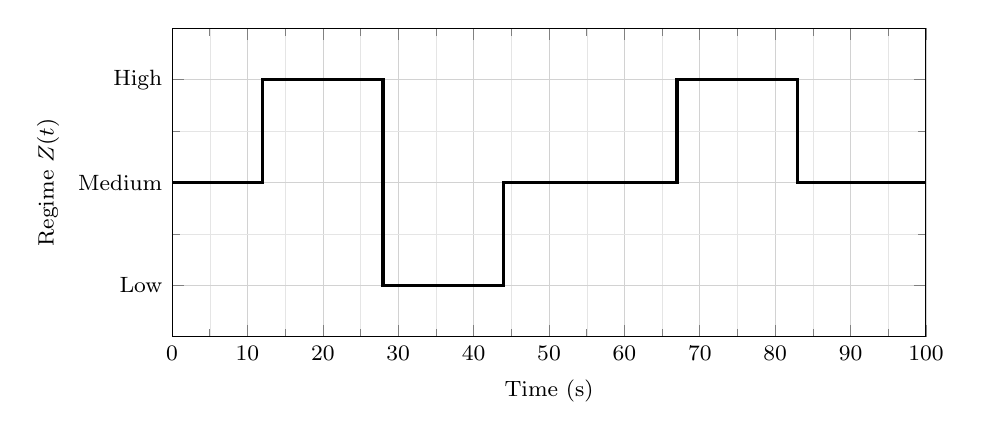
\begin{tikzpicture}
        \begin{axis}[
          width=0.92\linewidth,
          height=5.5cm,
          xmin=0, xmax=100,
          ymin=-0.5, ymax=2.5,
          xlabel={Time (s)},
          ylabel={Regime $Z(t)$},
          ytick={0,1,2},
          yticklabels={Low, Medium, High},
          grid=both,
          major grid style={line width=.2pt, draw=gray!35},
          minor grid style={line width=.1pt, draw=gray!20},
          minor tick num=1,
          ticklabel style={font=\footnotesize},
          label style={font=\footnotesize},
        ]
        \addplot[const plot, line width=1.2pt] coordinates {
          (0,1)   (12,1) (12,2)  (28,2) (28,0)  (44,0)
          (44,1)  (67,1) (67,2)  (83,2) (83,1)  (100,1)
        };
        \end{axis}
    \end{tikzpicture}
    \caption{Example of a regime-switching trajectory $Z(t)$ representing non-stationary environmental changes (e.g., traffic load levels).}
    \label{fig:regime_step_sem_inercia}
\end{figure}

Furthermore, to model the physical inertia of system responses (e.g., queue buildup or thermal throttling), we map the discrete regime target $u(t)$ to an observable variable $y(t)$ using a first-order dynamic equation:
\begin{equation}
    y_{k+1} = \alpha y_k + (1-\alpha)u_k
\end{equation}
where $\alpha \in [0,1)$ is the inertia factor. Figure \ref{fig:regime_com_inercia} shows how this results in smooth transitions, mimicking realistic metrics.

\begin{figure}[ht!]
    \centering
    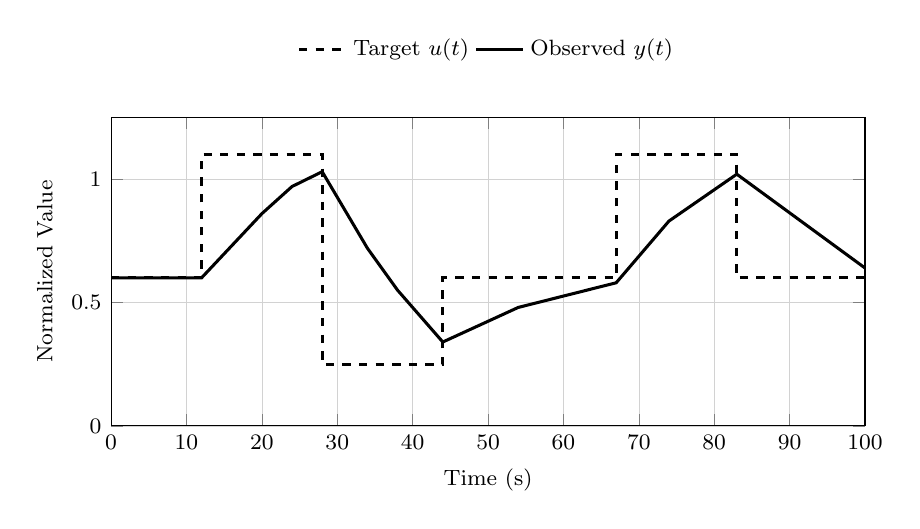
\begin{tikzpicture}
        \begin{axis}[
          width=0.92\linewidth,
          height=5.5cm,
          xmin=0, xmax=100,
          ymin=0, ymax=1.25,
          xlabel={Time (s)},
          ylabel={Normalized Value},
          grid=both,
          major grid style={line width=.2pt, draw=gray!35},
          minor grid style={line width=.1pt, draw=gray!20},
          legend style={at={(0.5,1.15)}, anchor=south, legend columns=2, draw=none, fill=none, font=\footnotesize},
          ticklabel style={font=\footnotesize},
          label style={font=\footnotesize},
        ]
        \addplot[const plot, line width=1.1pt, dashed] coordinates {
          (0,0.60)  (12,0.60) (12,1.10) (28,1.10) (28,0.25) (44,0.25)
          (44,0.60) (67,0.60) (67,1.10) (83,1.10) (83,0.60) (100,0.60)
        };
        \addlegendentry{Target $u(t)$}
        \addplot[line width=1.1pt] coordinates {
          (0,0.60) (12,0.60) (16,0.73) (20,0.86) (24,0.97) (28,1.03)
          (34,0.72) (38,0.55) (44,0.34) (54,0.48) (67,0.58) (74,0.83) (83,1.02) (100,0.64)
        };
        \addlegendentry{Observed $y(t)$}
        \end{axis}
    \end{tikzpicture}
    \caption{System response $y(t)$ with inertia tracking the regime target $u(t)$, avoiding unrealistic instantaneous jumps.}
    \label{fig:regime_com_inercia}
\end{figure}

\section{Proposed Solution}\label{sec_methodology}


\subsection{Fuzzy Logic}

\subsubsection{Fuzzification}

\subsubsection{Fuzzy Rules and Inference}

\subsection{Deep Reinforcement Learning Agent}

\subsubsection{State Space ($S_t$)}

\subsubsection{Action Space ($A_t$)}

\subsubsection{Reward Function ($R_t$)}

\section{Experimental Evaluation}\label{sec_experiments}

\subsection{Simulation Setup}


\section{Conclusion}\label{sec_conclusion}

\bibliographystyle{sn-mathphys-num}
\bibliography{bib/refs}

\end{document}
